\documentclass[a4paper,14pt]{extarticle}

\newcommand{\stend}{\textbf{Wb-demo-kit v.2}}

% Путь до папки с общими шаблонами
\newcommand{\pathToCommonFolder}{/home/denilai/Documents/repos/latex/Common}

% Название работы в титуле
\newcommand{\workname}{Отчет по практическим работам}
% Название дисциплины в титуле
\newcommand{\discipline}{Проектирование информационных систем}
% Название кафедры в титуле
\newcommand{\kafedra}{Кафедра инструментального и прикладного программного обеспечения}
% Тема работы в титуле
\newcommand{\theme}{Формирование требований к системе}
% Должность преподавателя в титуле
\newcommand{\rang}{ассистент}

% ФИО студента в титуле
\newcommand{\studentfio}{К.~Ю.~Денисов}%\\Д.~Н.~Федосеев\\А.~М.~Сосунов}\\%К.~Ю.~Денисов\\%И.~А.~Кремнев
% ФИО преподавателя в титуле
\newcommand{\teacherfio}{А.~А.~Русляков}


\usepackage{tabularx}
\usepackage{lastpage}


\usepackage{booktabs}
\newcolumntype{b}{X}
\newcolumntype{s}{>{\hsize=.5\hsize}X}
\newcommand{\heading}[1]{\multicolumn{1}{|c|}{\textbf{#1}}}

% установка размера шрифта для всего документа
%\fontsize{20pt}{18pt}\selectfont
\usepackage{extsizes} % Возможность сделать 14-й шрифт

% Вставка заготовки преамбулы
% Этот шаблон документа разработан в 2014 году
% Данилом Фёдоровых (danil@fedorovykh.ru) 
% для использования в курсе 
% <<Документы и презентации в \LaTeX>>, записанном НИУ ВШЭ
% для Coursera.org: http://coursera.org/course/latex .
% Исходная версия шаблона --- 
% https://www.writelatex.com/coursera/latex/5.3

% В этом документе преамбула

% Для корректного использования русских символов в формулах
% пакеты hyperref и настройки, связанные с ним, стоит загуржать
% перед загрузкой пакета mathtext



% поддержка русских букв
% кодировка шрифта
%\usepackage[T2A]{fontenc} 
\usepackage{pscyr}

% использование ненумеровонного абзаца с добавлением его в содержаниеl

\newcommand{\anonsection}[1]{\section*{#1}\addcontentsline{toc}{section}{#1}}
\newcommand{\sectionunderl}[1]{\section*{\underline{#1}}}


% настройка окружения enumerate
\usepackage{enumitem}
\setlist{noitemsep}
\setlist[enumerate]{labelsep=*, leftmargin=1.5pc}

\usepackage{hyperref}

% сначала ставить \usepackage{extsizes} % Возможность сделать 14-й шрифт
% для корректной установки полей вставлять преамбулу следует в последнюю очередь (но перед дерективой замены \rmdefault)
\usepackage[top=20mm,bottom=25mm,left=35mm,right=20mm]{geometry} % Простой способ задавать поля

\hypersetup{				% Гиперссылки
	unicode=true,           % русские буквы в раздела PDF
	pdftitle={Заголовок},   % Заголовок
	pdfauthor={Автор},      % Автор
	pdfsubject={Тема},      % Тема
	pdfcreator={Создатель}, % Создатель
	pdfproducer={Производитель}, % Производитель
	pdfkeywords={keyword1} {key2} {key3}, % Ключевые слова
	colorlinks=true,       	% false: ссылки в рамках; true: цветные ссылки
	linkcolor=red,          % внутренние ссылки
	citecolor=black,        % на библиографию
	filecolor=magenta,      % на файлы
	urlcolor=blue           % на URL
}

%%% Работа с русским языком
\usepackage{cmap}					% поиск в PDF
\usepackage{mathtext} 				% русские буквы в формулах
\usepackage[T2A]{fontenc}			% кодировка
\usepackage[utf8]{inputenc}			% кодировка исходного текста
\usepackage[english,russian]{babel}	% локализация и переносы
\usepackage{indentfirst}
\frenchspacing

%для изменения названия списка иллюстраций
\usepackage{tocloft}


\renewcommand{\epsilon}{\ensuremath{\varepsilon}}
\renewcommand{\phi}{\ensuremath{\varphi}}
\renewcommand{\kappa}{\ensuremath{\varkappa}}
\renewcommand{\le}{\ensuremath{\leqslant}}
\renewcommand{\leq}{\ensuremath{\leqslant}}
\renewcommand{\ge}{\ensuremath{\geqslant}}
\renewcommand{\geq}{\ensuremath{\geqslant}}
\renewcommand{\emptyset}{\varnothing}

% Изменения параметров списка иллюстраций
\renewcommand{\cftfigfont}{Рисунок } % добавляем везде "Рисунок" перед номером
\addto\captionsrussian{\renewcommand\listfigurename{Список иллюстративного материала}}

\newcommand{\tm}{\texttrademark\ }
\newcommand{\reg}{\textregistered\ }


%%% Дополнительная работа с математикой
\usepackage{amsmath,amsfonts,amssymb,amsthm,mathtools} % AMS
\usepackage{icomma} % "Умная" запятая: $0,2$ --- число, $0, 2$ --- перечисление

%% Номера формул
%\mathtoolsset{showonlyrefs=true} % Показывать номера только у тех формул, на которые есть \eqref{} в тексте.
%\usepackage{leqno} % Нумереация формул слева

%% Свои команды
\DeclareMathOperator{\sgn}{\mathop{sgn}}

%% Перенос знаков в формулах (по Львовскому)
\newcommand*{\hm}[1]{#1\nobreak\discretionary{}
{\hbox{$\mathsurround=0pt #1$}}{}}


% отступ для первого абзаца главы или параграфа
%\usepackage{indentfirst}

%%% Работа с картинками
\usepackage{graphicx}  % Для вставки рисунков
\graphicspath{{images/}{screnshots/}}  % папки с картинками
\DeclareGraphicsExtensions{.pdf,.png,.jpg}
\setlength\fboxsep{3pt} % Отступ рамки \fbox{} от рисунка
\setlength\fboxrule{1pt} % Толщина линий рамки \fbox{}
\usepackage{wrapfig} % Обтекание рисунков текстом

%%% Работа с таблицами
\usepackage{array,tabularx,tabulary,booktabs} % Дополнительная работа с таблицами
\usepackage{longtable}  % Длинные таблицы
\usepackage{multirow} % Слияние строк в таблице

%%% Теоремы
\theoremstyle{plain} % Это стиль по умолчанию, его можно не переопределять.
\newtheorem{theorem}{Теорема}[section]
\newtheorem{proposition}[theorem]{Утверждение}

\theoremstyle{plain} % Это стиль по умолчанию, его можно не переопределять.
\newtheorem{work}{Практическая работа}[part]


 
 
\theoremstyle{definition} % "Определение"
\newtheorem{corollary}{Следствие}[theorem]
\newtheorem{problem}{Задача}[section]
 
\theoremstyle{remark} % "Примечание"
\newtheorem*{nonum}{Решение}



%%% Программирование
\usepackage{etoolbox} % логические операторы

%%% Страница

%	\usepackage{fancyhdr} % Колонтитулы
% 	\pagestyle{fancy}
%   \renewcommand{\headrulewidth}{0pt}  % Толщина линейки, отчеркивающей верхний колонтитул
% 	\lfoot{Нижний левый}
% 	\rfoot{Нижний правый}
% 	\rhead{Верхний правый}
% 	\chead{Верхний в центре}
% 	\lhead{Верхний левый}
%	\cfoot{Нижний в центре} % По умолчанию здесь номер страницы

\usepackage{setspace} % Интерлиньяж
\onehalfspacing % Интерлиньяж 1.5
%\doublespacing % Интерлиньяж 2
%\singlespacing % Интерлиньяж 1

\usepackage{lastpage} % Узнать, сколько всего страниц в документе.

\usepackage{soul} % Модификаторы начертания


\usepackage[usenames,dvipsnames,svgnames,table,rgb]{xcolor}


\usepackage{csquotes} % Еще инструменты для ссылок

%\usepackage[style=authoryear,maxcitenames=2,backend=biber,sorting=nty]{biblatex}

\usepackage{multicol} % Несколько колонок

\usepackage{tikz} % Работа с графикой
\usepackage{pgfplots}
\usepackage{pgfplotstable}

% модуль для вставки рыбы
\usepackage{blindtext}

\usepackage{listings}
\usepackage{color}


% для поворота отдельной страницы. Использовать окружение \landscape
\usepackage{pdflscape} 
\usepackage{rotating} 


\definecolor{mygreen}{rgb}{0,0.6,0}
\definecolor{mygray}{rgb}{0.5,0.5,0.5}
\definecolor{mymauve}{rgb}{0.58,0,0.82}


% пример импорта файла
%\lstinputlisting{/home/denilai/repomy/conf/distributions}

\lstset{
	language=Python,
	basicstyle=\footnotesize,        % the size of the fonts that are used for the code
	numbers=left,                    % where to put the line-numbers; possible values are (none, left, right)
	numbersep=5pt,                   % how far the line-numbers are from the code
	numberstyle=\tiny\color{mygray}, % the style that is used for the line-numbers
	stepnumber=2,                    % the step between two line-numbers. If it's 1, each line will be numbered
	% Tab - 2 пробела
	tabsize=2,    
	% Автоматический перенос строк
	breaklines=true,
	frame=single,
	breakatwhitespace=true,
	title=\lstname 
}



\author{Кирилл Денисов}
\title{Лабораторная работа №1}
\date{\today}

\setcounter{withouttheme}{1}
\setcounter{withoutsubmissiondate}{0}

%если нужна тема работы в отчете, то указать в скобках что-либо, иначе оаставить пустым
%\renewcommand{\withouttheme}{}
%если нужна дата представления отчета, то указать в скобках что-либо
%\renewcommand{\withoutsubmissiondate}{1}

% установка полуторного интервала
% \usepackage{setspace}  
% \onehalfspacing

% использовать Times New Roman
\renewcommand{\rmdefault}{ftm}


\newcommand{\tb}{ThingsBoard~}

\begin{document}
	\thispagestyle{empty}
	% Вставка первого титульного листа
	% Есть две версии титульного листа - одиночный (titul) и групповой (titulAll)
	%\newcounter{withouttheme}

%\setcounter{withouttheme}{<n>} установить значение счетчика  withouttheme для определения, нужна ли тема
%    {0} - нужна
%    {1} - не нужна

%\setcounter{withoutsubmissiondate}{<n>} установить значение счетчика  withoutsubmissiondate для определения, нужна ли дата представления к защите
%     {0} - нужна
%     {1} - не нужена
\begin{center}
	\begin{figure}[h!]
		\begin{center}
		%\vspace{-10ex}
		
\includegraphics[width=0.17\linewidth]{\pathToCommonFolder/gerb}
		%\caption{}\label{pic:first}
		%	\vspace{5ex}
		\end{center}	
	\end{figure}
 	\small	МИНОБРНАУКИ РОССИИ \\
	Федеральное государственное бюджетное образовательное учреждение\\
						высшего образования\\
\normalsize					
\textbf{«МИРЭА – Российский технологический университет»\\
						РТУ МИРЭА}\\
						\noindent\rule{1\linewidth}{1pt}\\
       Институт информационных технологий\\ %\vspace{2ex}
					\kafedra\\
		\vspace{3ex}
			\large \textbf{\workname}  \\
		%\vspace{1ex}
						по дисциплине\\ «\discipline» \\
		\vspace{3ex}
		\ifnum \value{withouttheme}=0 {
			\textbf{Тема работы:}\\ <<\theme>>
		}
		\else {}
		\fi
\vspace{10ex}
\small
\begin{table}[h!]
\begin{tabular}{lp{0.6\linewidth}l}
	\textbf{Выполнил:} & студент группы ИВБО-02-19 & \\ 
	& & \studentfio \\%Д.~Н.~Федосеев\\%А.~М.~Сосунов\\%К.~Ю.~Денисов\\%И.~А.~Кремнев
	\textbf{Принял:} & \rang & \\
	& & \teacherfio \hfill\\
\end{tabular}
\end{table}
\end{center}
\ifnum \value{withoutsubmissiondate}=0 {
	\begin{flushleft}
		Работа представлена к защите <<\rule{3ex}{1pt}>>\rule{10ex}{1pt} 202\rule{1ex}{1pt} г.\hfill
	\end{flushleft}
\else {}
\fi

\normalsize
\begin{center}	
\vfill
Москва 2022
\end{center}

	\newpage
	\tableofcontents
	\newpage
	%\listoftables
	
\normalsize

\section{Формирование требований к системе}
\subsection{РЕФЕРАТ}
Суть данной практической работы заключается в анализе и формировании требований к разрабатываемой информационной системе <<Электронный сборник лабораторных работ>>, в том числе требований к составу и содержанию работ по подготовке объекта автоматизации к вводу системы в действие, а также требований к документированию определении и формализации бизнес-ролей.

Данная практическая работа содержит
\pageref*{LastPage}~страницы
%, \totfig~рисунков
% \tottab~таблицы.

%\newpage
\subsection{ОПИСАНИЕ ОБЪЕКТА АВТОМАТИЗАЦИИ}

Разрабатываемая информационная система <<Электронный сборник лабораторных работ>> (далее по тексту Система) служит для сбора, хранения и учета письменных работ различного характера, выполненных учащимися средних общеобразовательных, средних специальных и высших учебных заведений. На данной платформе пользователям на безвозмездной основе предоставляется доступ к загруженным документам, топикам и темам форума и медиафайлам. 

Система выполняет функции образовательной платформы. Платформа может быть интегрирована в информационную среду учебных заведений, предоставляя инструменты для учета и хранения работ учащихся. 

%\newpage
\subsection{ОБЩИЕ СВЕДЕНИЯ}
\subsubsection{Список требований и определений}

Подсистема управления доступом (ПУД) --- часть Системы, назначающая разрешения конечным пользователям в зависимости от их роли в вашей организации. ПУД обеспечивает гранулярный контроль, предлагая простой и управляемый подход к управлению доступом, который менее подвержен ошибкам, чем индивидуальное назначение разрешений.

\subsubsection{Описание бизнес-ролей}
\begin{table}[h!]
	\caption{Описание бизнес-ролей}\label{tab:roles}
	\begin{tabular}{|l|p{0.6\linewidth}|}
		\hline 
		\multicolumn{1}{|c|}{\textbf{Бизнес-роль}} & \multicolumn{1}{c|}{\textbf{Описание}}\\ \hline\hline
		Администратор системы & Лицо, имеющее доступ к ПУД и другим инструментам администрирования Системы \\ \hline
		Пользователь & Лицо или организация, которая использует Систему для размещения и хранения файлов, имеет личный кабинет на портале, может участвовать в обсуждениях на форуме\\ \hline
	\end{tabular}
\end{table}


%\newpage
\subsection{ТРЕБОВАНИЯ К СИСТЕМЕ}
\subsubsection{Бизнес требования}

Система должна предоставлять функционал для удобного удаленного хранения и управления электронными документами.

Использование системы в качестве хранилища должно быть более привлекательно, чем хранение файлов на локальном компьютере или физическом носителе.

Система должна иметь возможность быть интегрированной в информационную платформу общеобразовательных учреждений.


\subsubsection{Пользовательские требования}
Пользователь должен иметь возможность авторизоваться в системе для загрузки документов в хранилище.

Пользователь должен иметь возможность скачивания файлов без ограничений и необходимости регистрации .

Пользователь должен иметь возможность оставлять отзыв и оценку конкретному документу, размещенному в системе.

Пользователь должен иметь возможность создать тему на портале.

\subsubsection{Функциональные требования}

Система должна отвечать требованиям по хранению, обработке и защите персональных данных в соответствии с 152-ФЗ «О персональных данных».

Система должна иметь упорядоченную структуру файлов с разделением по языкам, научным дисциплинам, видам работ.

Данные должны хранится в течение 20 лет.

В системе должен сочетаться функционал хранилища данных и образовательного форума.

Платформа должна реализовывать систему управления (авторизации) доступом на основе ролей.

Система должна реализовывать функционал по аутентификации пользователя по логину (почтовому адресу) и паролю.

Персональные данные пользователя и хеш-строки паролей должны храниться в зашифрованном виде.

К загрузке должны допускаться файлы любого формата.

\subsubsection{Нефункциональные требования}

В качестве алгоритма хеширования должен использоваться SHA-256.

Система должна представлять собой интернет-ресурс, разработанный в среде разработки Bitrix Framework.

Каждому пользователю должно предоставляться персональное хранилище данных в размере 5 ГБ с возможностью расширения. 

Для хранения сведений о пользователях системы, записях образовательного форума и метаданных используется база данных под управлением PostgreSQL.

Для хранения пользовательских файлов должно использоваться хранилище блочного типа. Файлы в таком хранилище делятся на блоки равного размера и размещаются в памяти сервера. По запросу платформы система хранения собирает файл из блоков, используя метаданные.

\subsubsection{Требования к пользовательскому интерфейсу}
Пользовательский интерфейс должен содержать нейтральные цвета и
контрастный, хорошо читаемый текст. Основные цвета --- белый, синий.

Обязательными элементами пользовательская  являются:

\textbf{Наличие функции поиска}.

 Является обязательным условием каждого крупного веб-проекта, состоящего более чем из 10-и страниц.
	
	Реализация простого поиска, позволяющий находить нужную информацию по ключевым запросам. Поисковое окно располагается в верхней части сайта и проходит через все страницы сайта.
	
\textbf{Меню}
	
	Список доступных разделов и категорий должен быть всегда заметен пользователю, независимо от его местонахождения на сайте. Следовательно, пользователь всегда должен видеть возможные варианты переходов.
	Кроме того, подобное «сквозное» меню упрощает индексацию сайта для поисковых машин, способствует равномерному распределению «веса» между всеми страницами сайта.
	
	Веб-интерфейс должен содержать элементы управления и манипуляции документами, вкладки и разделы, отведенные под форум.
	
	 \textbf{Адаптивный дизайн}
	
	Дизайн веб-страниц должен обеспечивать правильное отображение сайта на различных устройствах, подключённых к интернету и динамически подстраиваться под заданные размеры окна браузера.
	
	Сайт может работать на смартфоне, планшете, ноутбуке и телевизоре с выходом в интернет, то есть практически на всем спектре устройств.
	
\subsubsection{Требования к защите информации}
Для обеспечения защиты информации от несанкционированного доступа требуется реализация следующих функций:

\paragraph*{В части управления доступом:}

\begin{itemize}
	\item  должна осуществляться идентификация и проверка подлинности субъектов доступа при входе в Систему по идентификатору (коду) и паролю условно-постоянного действия длиной не менее шести символов;
	
	\item должна осуществляться идентификация АРМ, серверов, каналов связи, внешних устройств ЭВМ по логическим именам;
	
	\item должен осуществляться контроль доступа субъектов к защищаемым ресурсам в соответствии с ролевой моделью.
\end{itemize}
\paragraph*{В части регуляции и учета:}
\begin{itemize}
	\item  должна осуществляться регистрация входа/выхода субъектов доступа в систему/из системы.
	\item В параметрах регистрации должны указываться:
	\subitem время и дата входа/выхода субъекта доступа в систему/из системы
	\subitem идентификатор (код или фамилия) субъекта, предъявленный при попытке доступа;
\end{itemize}

\subsubsection{Требования по сохранности информации при авариях}
Сохранность информации в Системе должна обеспечиваться при следующих аварийных ситуациях:
\begin{itemize}
	\item импульсные помехи, сбои и перерывы в электропитании;
	\item нарушение или выход из строя каналов связи локальной сети;
	\item сбой общего или специального программного обеспечения (сервера);
	\item ошибки в работе персонала
\end{itemize}


\subsubsection{Требования по стандартизации и унификации}
Для работы с БД должен использоваться язык SQL в рамках стандарта ANSI SQL-92.

Для разработки пользовательского интерфейса и средств генерации отчетов (любых твердых копий) должны использоваться языки 4-го поколения.

При создании Системы должно использоваться стандартное общее программное обеспечение, включающее лицензионные ОС, СУБД, сетевую операционную систему.



\subsubsection{Требования к безопасности}
Система не должна выдавать варианты, которые потенциально могут
усугубить состояние оборудования.

Система должна выдавать пользователю правила технической безопасности, которые ему необходимо принять, чтобы пользоваться системой.

Системой должен осуществляться контроль доступа к конфиденциальным данным.

Должны предприниматься шаги, направленные на предотвращение утечек персональных данных пользователей Системы.

Система должна быть защищена от внешних атак.

\subsubsection{Требования к документированию}
Проектная документация должна быть разработана в соответствии с
ГОСТ 34.201-89 и ГОСТ 7.32-2017.

Отчетные материалы должны включать в себя текстовые материалы
(представленные в виде бумажной копии и на цифровом носителе) и графические материалы.

Предоставить следующие документы:

\begin{enumerate}
	\item Схема функциональной структуры автоматизируемой деятельности.
	\item  Описание технологического процесса обработки данных.
	\item  Описание информационного обеспечения.
	\item  Описание программного обеспечения АС.
	\item  Схема логической структуры БД.
	\item  Руководство пользователя.
	\item  Описание контрольного примера (по ГОСТ 24.102).
	\item  Протокол испытаний (по ГОСТ 24.102).
	
\end{enumerate}

%\newpage
\subsubsection{Требования к функциям, выполняемым системой}
\begin{table}[h!]
	\caption{\label{tab:functions} Требования к функциям, выполняемым системой.}
	\begin{center}\small
		\begin{tabular}{|m{0.4\linewidth}|m{0.4\linewidth}|}
			\hline
			\heading{Функция} & \heading{Задача}\\
			\hline
			
			\multirow{2}{0.95\linewidth}{Работа с пользователями}
			& Регистрация пользователя \\\cline{2-2}
			& Авторизация пользователя \\\hline

			\multirow{4}{0.95\linewidth}{Добавление новых документов в хранилище данных} 
			& Заполнение сведений о документе \\\cline{2-2}
			& Загрузка документа в объектное хранилище данных \\\cline{2-2}
			& Обновление сведений о документах пользователя \\\cline{2-2}
			& Проведение проверки и корректировку связей в хранилище метаданных \\\hline
			
			\multirow{4}{0.95\linewidth}{Загрузка документов из хранилища данных} 
			& Запрос сведений о документе \\\cline{2-2}
			& Выгрузка документа из объектного хранилища данных \\\cline{2-2}
			& Выдача результата пользователю \\\cline{2-2}
			& Проведение проверки и корректировку связей в хранилище метаданных \\\hline
			
			
		\end{tabular}
	\end{center}
\end{table}
%\newpage
\subsection{СЦЕНАРИИ ИСПОЛЬЗОВАНИЯ}


\begin{enumerate}
	\item Пользователь заходит на веб ресурс с целью ознакомления с содержанием или скачивания интересующего его документа. Он может оценить размещенный документ, оставив отметку «Нравится». Также пользователь может получить цифровую копию документа не проходя аутентификацию в системе. 
	\item Пользователь заходит на веб-ресурс с целью загрузки документа. Для этого ему необходимо пройти регистрацию в Системе. После этого пользователь получит доступ к личному кабинету и персональному хранилищу данных размером 5 ГБ.
	\item Пользователь заходит на веб-ресурс с целью заведения темы на форуме, входящем в состав Системы. Для этого ему необходимо пройти регистрацию в Системе. После этого пользователь получит доступ к личному кабинету и получит возможность оставлять комментарии под записями на форуме, создавать новые темы для обсуждения.
\end{enumerate}

\newpage
\section{Выбор архитектуры системы}

\subsection{ФУНКЦИОНАЛЬНЫЕ СХЕМЫ СИСТЕМЫы}
В ходе данной практической работы были разработаны три различные функциональные схемы для реализации информационной системы <<Электронный сборник лабораторных работ>>.


Архитектура информационной системы --- концепция,
определяющая модель, структуру, выполняемые функции и
взаимосвязь компонентов информационной системы.
Можно сформулировать проще:
Информационная система --- это совокупность программного
обеспечения, решающего определенную прикладную задачу.


Архитектура информационной системы --- абстрактное
понятие, определяющее, из каких составных частей (элементов,
компонент) состоит приложение и как эти части между собой
взаимодействуют.



\subsubsection{Распределенная архитектура}


Ключевое отличие данной архитектуры --- абстрагирование от физической схемы данных и манипулирование
данными клиентскими программами на уровне логической схемы. Это позволило создавать надежные многопользовательские информационные системы с
централизованной базой данных, независимые от аппаратной (а
часто и программной) части сервера базы данных и поддерживающие
графический интерфейс пользователя на клиентских станциях,
связанных локальной сетью. 

% TODO: \usepackage{graphicx} required
\begin{figure}[h!]
	\centering
	\includegraphics[width=0.7\linewidth]{"disterbute"}
	\caption{Распределенная архитектура системы}
	\label{fig:disterbute}
\end{figure}


\subsubsection{Клиент-серверная архитектура}
На рисунке 2.3 представлена схема клиент-серверной архитектуры разрабатываемой  системы.
Все подсистемы можно разбить на 2 группы: подсистемы серверной части и подсистемы клиентской части. 

Серверная часть системы включает в себя подсистему БД и подсистему обработки запросов сетевого протокола HTTPS. Подсистема БД содержит СУБД, выполняющую запросы к БД, саму БД, также система должна выполнять резервное копирование данных. Подсистема обработки запросов призвана обрабатывать HTTPS запросы, поступающие от клиентов, и формировать запросы к БД в соответствии с целью запроса.
Подсистемы ЛКС и контроля успеваемости предназначены для обеспечения диалога между системой и пользователями 2 групп: студентов и сотрудников деканата. Подсистемы имеют графический интерфейс, что облегчает взаимодействие пользователей с системой в целом. Подсистемы также автоматически собирают и отправляют HTTPS запросы в соответствии с нуждами и действиями пользователя.


Оособенности:
\begin{enumerate}
	\item  клиентская программа работает с данными через запросы к
	серверному ПО;
	14
	\item  базовые функции приложения разделены между клиентом и
	сервером.
	Положительные стороны:
	\item  полная поддержка многопользовательской работы;
	\item  гарантия целостности данных.
	Отрицательные стороны:
	\item  Бизнес логика приложений осталась в клиентском ПО. При
	любом изменении алгоритмов, надо обновлять пользовательское
	ПО на каждом клиенте.
	\item  Высокие требования к пропускной способности
	коммуникационных каналов с сервером.
	\item  Слабая защита данных от взлома, в особенности от
	недобросовестных пользователей системы.
	\item  Высокая сложность администрирования и настройки рабочих
	мест пользователей системы.
	\item  Необходимость использовать мощные ПК на клиентских местах.
	\item  Высокая сложность разработки системы из-за необходимости
	выполнять бизнес-логику и обеспечивать пользовательский
	интерфейс в одной программе.
\end{enumerate}

% TODO: \usepackage{graphicx} required
\begin{figure}[h!]
	\centering
	\includegraphics[width=0.8\linewidth]{client-server"}
	\caption{Клиент-серверная архитектура системы}
	\label{fig:client-server}
\end{figure}

\subsection{ВЫБОР АРХИТЕКТУРЫ}

В ходе выполнения данной практической работы были предложены две различные функциональные схемы системы.
Проанализировав каждую из них, можно сделать вывод, что оптимальным вариантом является система с клиент-серверной архитектурой. Основанием для такого заключения являются следующие характеристики:
\begin{itemize}
	\item  наличие графического интерфейса пользователя;
	\item зашифрованная передача запросов по протоколу HTTPS.
\end{itemize}
Графический интерфейс позволит работать с системой <<Электронный сборник лабораторных работ>> даже пользователям, не имеющих специфических навыков работы с компьютером, т.е. навыки взаимодействия, например, с СУБД не требуются. Защищенное соединение по протоколу HTTPS обеспечит дополнительную защиту данных при передаче их по сети Интернет.

\newpage
\section{Функциональное проектирование\\(методология SADT)}
\subsection{ЦЕЛЬ СОЗДАНИЯ СИСТЕМЫ}
Разрабатываемая информационная система <<Электронный сборник лабораторных работ>> (далее по тексту Система) служит для сбора, хранения и учета письменных работ различного характера, выполненных учащимися средних общеобразовательных, средних специальных и высших учебных заведений. На данной платформе пользователям на безвозмездной основе предоставляется доступ к загруженным документам, топикам и темам форума и медиафайлам. 

Система выполняет функции образовательной платформы. Платформа может быть интегрирована в информационную среду учебных заведений, предоставляя инструменты для учета и хранения работ учащихся. 


\subsection{КРАТКОЕ ОПИСАНИЕ}

Пользователь взаимодействует с системой посредством веб-сервиса.  Сайт является удобным
интернет сервисом, представляющим информацию о персональных файлах, перечне загруженных в Систему работ. Веб-интерфейс реализует возможность доступа к форуму для обсуждений. Для комфортного и
круглосуточного доступа, сайт так же адаптирован для мобильных устройств.

Кроме того, платформа позволяет пользователю просматривать файлы, основываясь на большом количестве поисковых фильтров. Сортировка возможна по времени загрузки, наименованию научной дисциплины, виду и популярности работы.


\subsection{СРЕДСТВА СОЗДАНИЯ ИС}
В качестве средств создания ИС был использован язык программирования PHP и JavaScript. Для хранения метаданных и системных сообщений используется база данных под управлением СУБД PostreSQL. Для хранения пользовательских файлов используется объектное хранилище S3.

В качестве инструмента веб-аналитики используется Яндек.Метрика. Данных инструмент помогает получать наглядные отчеты, видеозаписи действий посетителей, отслеживать источники трафика и оценивать эффективность онлайн- и офлайн-рекламы.

Система построена в соответствии с подходом Ajax, заключающийся в <<фоновом>> обмене данными браузера с веб-сервером. В результате при обновлении данных веб-страница не перезагружается полностью, и веб-приложения становятся быстрее и удобнее.

Для моделирования проектируемой ИС будет
использоваться нотация IDEF0 программном обеспечении CASE Ramus
Educational edition.

\subsection{ПРОЕКТИРОВАНИЕ КОНТЕКСТНОЙ ДИАГРАММЫ}

Была спроектирована контекстная диаграмма A-0 в нотации IDEF0.
В качестве входа по управлению (стрелка управления) были выбраны
следующие нормативные и правовые документы:

\begin{enumerate}
	\item 152-ФЗ "О персональных данных".
	\item 149-ФЗ "Об информации, информационных технологиях и о защите информации".
	\item Политика интернет-сайта.
	\item Пользовательское соглашение.
\end{enumerate}

В качестве входящих информационных потоков, которые подлежат
обработке и преобразованию в процессе работы ИС была указана следующая
информация:
\begin{enumerate}
	\item Персональные данные пользователя
	\item Пользовательские файлы
\end{enumerate}

В качестве механизмов (ресурсов, выполняющих работу) были
выделены:
\begin{enumerate}
	\item Подсистема хранения.
	\item Подсистема обработки запросов.
	\item Подсистема технической поддержки.
	\item Подсистема личного кабинета.
	\item Подсистема форума.
	\item Модератор форума.
	\item Пользователь системы.
\end{enumerate}

В качестве выходов после выполнения ИС получены следующие
информационные элементы:
\begin{enumerate}
	\item Статистические данные об активности пользователей.
	\item Сведения о работе подсистем.
\end{enumerate}

Так как механизмы <<Подсистема хранения>>, <<Подсистема обработки запросов>> и <<Пользователь системы>> 
%и входы по управлению <<152-ФЗ 'О пероснальных данных'>> и <<149-ФЗ 'Об информации, информационных технологиях и о защите информации'>> 
используются во всех выделяемых в ходе дальнейшей декомпозиции процессов, то соответствующие стрелки туннелированы. На схеме оконечности данных стрелок заключены в круглые скобки.

% TODO: \usepackage{graphicx} required
\begin{figure}[h!]
	\centering
	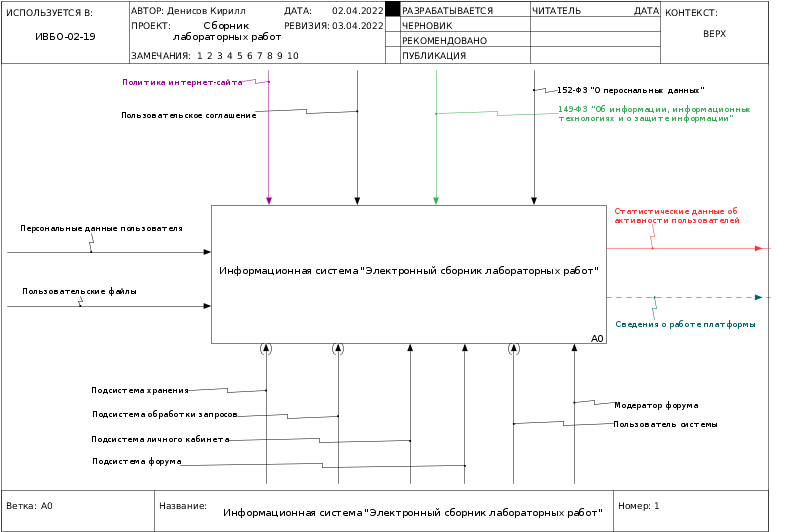
\includegraphics[width=\linewidth]{images/ramus/01_A0}
	\caption{Контекстная диаграмма процесса предоставления услуг сервисом "Сборник лабораторных работ"}
	\label{fig:01a0}
\end{figure}
\newpage


\section{Функциональное проектирование (нотация IDEF0)}
\subsection{ОПИСАНИЕ ПРОЦЕССОВ ДЕКОМПОЗИЦИИ}
На диаграмме уровня А0 декомпозиции функционального блока
<<Информационная система ''Электронный сборник лабораторных работ''>> обозначены процессы и функциональные блоки,
выполняемые в рамках процедуры:

\begin{enumerate}
	\item Процесс регистрации пользователя в системе.
	\item 	Процесс публикации файла в системе.
	\item Процесс получения файла, размещенного в системе.
	\item Процесс участия в обсуждении на форуме.
\end{enumerate}

Диаграмма декомпозиции блока <<Информационная система ''Электронный сборник лабораторных работ''>> приведена на рисунке~\ref{fig:02a0}.

% TODO: \usepackage{graphicx} required
\begin{figure}[h!]
	\centering
	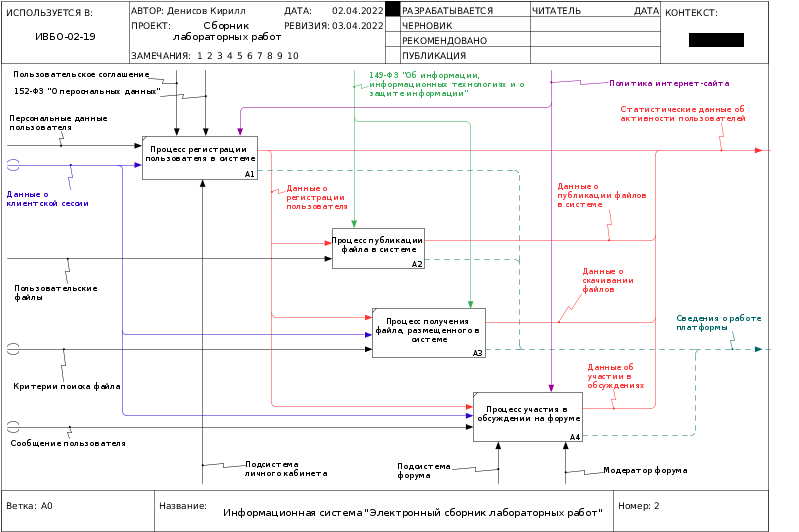
\includegraphics[width=\linewidth]{images/ramus/02_A0}
	\caption{Диаграмма декомпозиции}
	\label{fig:02a0}
\end{figure}


\subsubsection{Процесс регистрации пользователя в системе}

Процесс регистрации проходит согласно закону <<О персональных данных>> и политике интернет-сайта а также условиям, описанным в пользовательском соглашении.  
В качестве входных потоков выступают персональные данные пользователя и данные о клиентской сессии.
После регистрации пользователь может перейти к процессу публикации файлов или процессу получения файлов, размещенных на платформе. В качестве механизмов процесса выступают <<Подсистема хранения>> и <<Пользователь системы>>, а также <<Подсистема личного кабинета>>. Выходные потоки процесса --- данные о регистрации пользователя в системе и сведения о работе платформы (логи и метаданные подсистем).



\subsubsection{Процесс публикации файла в системе}
Процесс публикации файла в системе происходит в соответствии с федеральным законом <<Об информации, информационных технологиях и о защите информации>>, который оперирует понятиями <<объект авторского права>> и устанавливает правила распространения загружаемых объектов. В качестве входных потоков выступают данные о регистрации пользователя и данные о клиентской сессии. В качестве механизмов процесса выступают <<Подсистема хранения>> и <<Пользователь системы>>. Выходные потоки процесса --- данные о публикации файлов в системе и сведения о работе платформы (логи и метаданные подсистем).


\subsubsection{Процесс получения файла, размещенного в системе}
Процесс получения файла, размещенного в системе происходит в соответствии с федеральным законом <<Об информации, информационных технологиях и о защите информации>>, который оперирует понятиями <<объект авторского права>> и устанавливает правила распространения загружаемых объектов. В качестве входных потоков выступают данные о регистрации пользователя, данные о клиентской сессии и критерии поиска файла, предоставленные пользователем. В качестве механизмов процесса выступают <<Подсистема хранения>> и <<Пользователь системы>>. Выходные потоки процесса --- данные о скачивании файлов и сведения о работе платформы (логи и метаданные подсистем).


\subsubsection{Процесс участия в обсуждении на форуме}
Процесс участия в обсуждении на форуме происходит в соответствии с политикой интернет-сайта. Входные потоки процесса --- данные о регистрации пользователя, данные о клиентской сессии и сообщения пользователя.  В качестве механизмов процесса выступают <<Подсистема хранения>> и <<Пользователь системы>>, а также <<Подсистема форума>> и <<Модератор форума>>. Выходные потоки процесса --- данные об участии в обсуждениях и сведения о работе платформы (логи и метаданные подсистем).

\subsection{ДЕКОМПОЗИЦИЯ ФУНКЦИОНАЛЬНОГО БЛОКА}
Рассмотрим диаграмму процессов, происходящих в функциональном
блоке А2, приведенном выше

На рисунке \ref{fig:03a2} рассмотрена декомпозиция функционального блока А2.

% TODO: \usepackage{graphicx} required
\begin{figure}[h!]
	\centering
	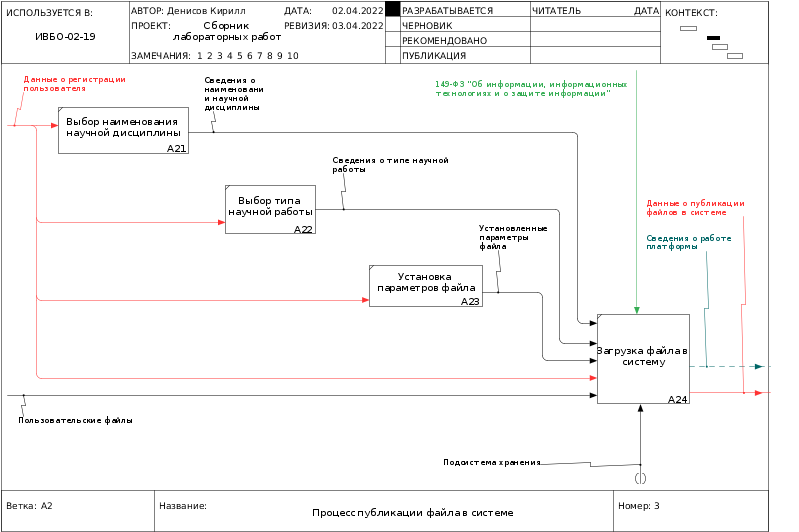
\includegraphics[width=0.9\linewidth]{images/ramus/03_A2}
	\caption{Диаграмма декомпозиции функционального блока А2.}
	\label{fig:03a2}
\end{figure}

Исходя из детального уточнения выполняемых задач ИС, были определены
следующие функциональные элементы:
\newpage
\begin{enumerate}
	\item Выбор наименования научной дисциплины.
	\item Выбор типа научной работы.
	\item Установка параметров файла.
	\item Загрузка файла в систему.
\end{enumerate}

Все процессы осуществляются пользователем с помощью <<Подсистемы обработки запросов>> системы <<Электронного сборника лабораторных работ>>.

\subsubsection{Выбор наименования научной дисциплины}
Процесс <<Выбор наименования научной дисциплины>> принимает в качестве входного потока данные о регистрации пользователя. Выходным потоком являются сведения о наименовании научной дисциплины. 


\subsubsection{Выбор типа научной работ}
Процесс <<Выбор типа научной работы>> принимает в качестве входного потока данные о регистрации пользователя. Выходным потоком являются сведения о типе научной работы.


\subsubsection{Установка параметров файла}
Процесс <<Установка параметров файла>> принимает в качестве входного потока данные о регистрации пользователя. Выходным потоком являются установленные параметры файла.


\subsubsection{Загрузка файла в систему}
Процесс <<Загрузка файла в систему>> в дополнение к механизмам <<Подсистема обработки запросов>> и <<Пользователь системы>> использует <<Подсистему хранения>>. В качестве входного потока данный процесс принимает сведения о регистрации пользователя, сведения о наименовании научной дисциплины, сведения о типе научной работы, установленные параметры файла и пользовательские файлы. Процесс проходит в соответствии с федеральным законом <<Об информации, информационных технологиях и о защите информации>>, который оперирует понятиями <<объект авторского права>> и устанавливает правила распространения загружаемых объектов.

\newpage
\section{Функциональное проектирование (нотация DFD)}

\subsection{ОПРЕДЕЛЕНИЕ ОБЪЕКТА ДЕКОМПОЗИЦИИ}
Для построение диаграммы в нотации DFD был выбран <<Процесс получения файла, размещенного в системе>>. 

Данный процесс был выбран, так как он реализует один из базовых функционалов системы и является технически сложным. 

В ходе данного процесса осуществляется обращение к нескольким хранилищам данных, а именно к хранилищу метаданных, содержащему сведения о предлагаемых к выбору наименованиях научных дисциплин, типах работ, параметрах файлов, хранящихся в объектном хранилище файлов, и к самому объектному хранилищу файлов.


Было выделено два основных процесса на диаграмме потоков данных:
\begin{enumerate}
	\item Установка критериев
	поиска в блоке фильтров.
	\item Обращение
	к хранилищу файлов.
\end{enumerate}
%\vspace{5ex}
\subsubsection{Установка критериев поиска}
В ходе первого процесса устанавливаются критерии поиска и фильтры файлов. В ходе данного процесса подсистема обработки запросов формирует запрос к хранилищу метаданных, получая список файлов, удовлетворяющих требованиям пользователя. 
\subsubsection{Обращение к хранилищу файлов}
В ходе второго процесса осуществляется доступ к хранилищу метаданных с целью получения сведений о расположении требуемого файла, затем инициализируется защищенное FTP соединение и пользователю предлагается скачать файл. 

Полученная схема в нотации DFD изображена на рисунке \ref{fig:dfd}.
% TODO: \usepackage{graphicx} required
\begin{figure}[h!]
	\centering
	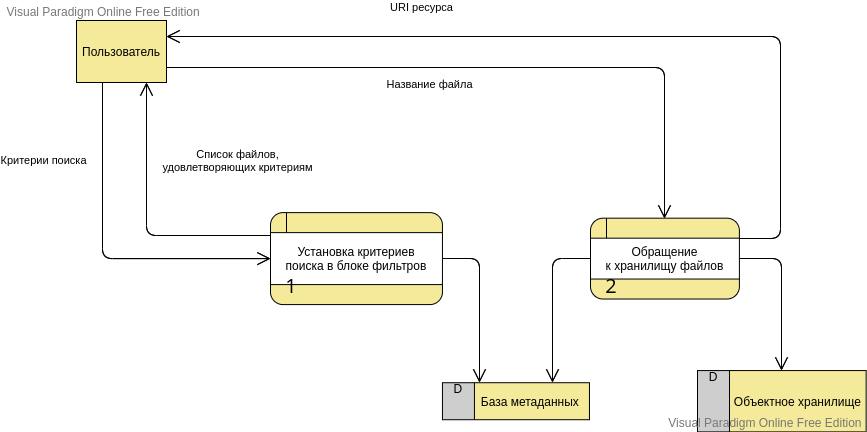
\includegraphics[width=0.9\linewidth]{images/dfd}
	\caption{Диаграмма потока данных}
	\label{fig:dfd}
\end{figure}
%\subsection{Вывод}
%В ходе выполнения данной практической работы была построена диаграмма потока данных, описывающая процесс скачивания файла, размещенного в информационной системе <<Электронный сборник лабораторных работ>>, уточнены сценарии взаимодействия с хранилищами метаданных и объектным хранилищем Подсистемы хранения.

\clearpage
\section{Проектирование структуры данных ИС (Entity Relation Diagram)}


%\section{Разработка диаграммы отношений (Entity Relation Diagram)}
%\subsection{Цель работы}
%Логическое моделирование ИС <<Электронный сборник лабораторных работ>>.
\subsection{МОДЕЛИРОВАНИЕ СИСТЕМЫ}
Для логического моделирования было выбрано программное обеспечение Draw.io в силу того, что оно предлагает удобный веб-интерфейс для работы а также реализует возможность создания диаграмм в различных нотациях. Данное программное обеспечение позволяет экспортировать файлы в формате, удобном для переноса между платформами и в виде изображений, что удобно при разработке документации, прилагаемой к реализуемой ИС.

\subsection{КРАТКАЯ ПОСТАНОВКА ЗАДАЧИ}
Главная задача системы --- сбор и обработка научных и ученических работ пользователей. Система должна представлять данные о файлах в структурированном виде, предлагать удобный интерфейс взаимодействия с личными файлами и представлять возможность получения файлов, хранящихся в системе.

Основываясь на поставленной задаче, была создана модель данных базы метаданных, обеспечивающей работу и обслуживание объектного хранилища, содержащего пользовательские файлы, загружаемые в систему.

Хранилище метаданных выполнено по схеме <<Звезда>>, где основная таблица фактов связана с несколькими таблицами измерений, организуя удобную для хранения многомерных показателей схему реалиционных таблиц.
%\newpage
В таблице фактов содержатся следующие данные:

\begin{table}[h!]
	\caption{Таблица фактов PaperFacts}
	\begin{tabular}{|p{0.3\linewidth}|p{0.6\linewidth}|}
		\hline
		\heading{Название} & \heading{Назначение} \\ \hline
		ID & Индефикатор записи \\ \hline
		paperID & Индефикатор документа \\ \hline
		authorID & Индефикатор автора \\ \hline
		disciplineID & Индефикатор дисциплины  \\ \hline
		work\_typeID & Индефикатор типа работы \\ \hline
		organizationID & Индефикатор организации \\ \hline
		licenseID & Индефикатор лицензии \\ \hline
		timestamp & Временная метка \\ \hline
		status & Статус для версионирования \\ \hline
		name & Название работы \\ \hline
	\end{tabular}
	\label{tab:facts}
\end{table}

В таблице измерения <<Авторы>> содержатся следующие данные:

\begin{table}[h!]
	\caption{Таблица измерения Authors}
	\begin{tabular}{|p{0.3\linewidth}|p{0.6\linewidth}|}
		\hline
		\heading{Название} & \heading{Назначение} \\ \hline
		authorID & Индефикатор автора \\ \hline
		firstname & Имя \\ \hline
		secondname & Фамилия \\ \hline
		degree & Степень (должность) \\ \hline
		nickname & Никнейм \\ \hline
		email & Адрес электронной почты \\ \hline
		country & Страна \\ \hline
		city & Город \\ \hline
	\end{tabular}
	\label{tab:authors}
\end{table}

В таблице измерения <<Организации>> содержатся следующие данные:
\begin{table}[h!]
	\caption{Таблица измерения Organizations}
	\begin{tabular}{|p{0.3\linewidth}|p{0.6\linewidth}|}
		\hline
		\heading{Название} & \heading{Назначение} \\ \hline
		organizationID & Индефикатор организации \\ \hline
		country & Страна \\ \hline
		city & Город \\ \hline
		type & Тип организации \\ \hline
		name & Название организации \\ \hline
	\end{tabular}
	\label{tab:orgs}
\end{table}

\newpage
В таблице измерения <<Лицензии>> содержатся следующие данные:
\begin{table}[h!]
	\caption{Таблица измерения Licenses}
	\begin{tabular}{|p{0.3\linewidth}|p{0.6\linewidth}|}
		\hline
		\heading{Название} & \heading{Назначение} \\ \hline
		licenseID & Индефикатор лицензии \\ \hline
		name & Название лицензии \\ \hline
		supervisor & Котролирующая организация \\ \hline
	\end{tabular}
	\label{tab:licenses}
\end{table}

В таблице измерения <<Типы работ>> содержатся следующие данные:
\begin{table}[h!]
	\caption{Таблица измерения WorkTypes}
	\begin{tabular}{|p{0.3\linewidth}|p{0.6\linewidth}|}
		\hline
		\heading{Название} & \heading{Назначение} \\ \hline
		work\_typeID & Индефикатор типа работы \\ \hline
		name & Название типа работы \\ \hline
	\end{tabular}
	\label{tab:worktypes}
\end{table}


В таблице измерения <<Работы>> содержатся следующие данные:
\begin{table}[h!]
	\caption{Таблица измерения Papers}
	\begin{tabular}{|p{0.3\linewidth}|p{0.6\linewidth}|}
		\hline
		\heading{Название} & \heading{Назначение} \\ \hline
		paperID & Индефикатор файла работы \\ \hline
		URI & Универсальный индефикатор ресурса \\ \hline
		status & Статус для версионирования \\ \hline
	\end{tabular}
	\label{tab:papers}
\end{table}

В таблице измерения <<Дисциплины>> содержатся следующие данные:
\begin{table}[h!]
	\caption{Таблица измерения Disciplines}
	\begin{tabular}{|p{0.3\linewidth}|p{0.6\linewidth}|}
		\hline
		\heading{Название} & \heading{Назначение} \\ \hline
		disciplineID & Индефикатор дисциплины  \\ \hline
		name & Название дисциплины \\ \hline
	\end{tabular}
	\label{tab:disciplines}
\end{table}

Таблица фактов поддерживает версионирование медленно изменяющихся измерений второго типа (SCD2). Версионирование нужно не для хранения разных версий одного файла в системе, а для отражения в базе данных факта изменения параметров файла. Например, при изменении типа работы запись об этом сохранится в базе, при этом это никак не скажется на доступности файла в объектном хранилище, так как ссылка на файловый ресурс не будет затронута.

\subsection{ПОСТРОЕНИЕ ER ДИАГРАММЫ}

ER диаграмма приведена на рисунке \ref{fig:data-model}.

% TODO: \usepackage{graphicx} required
\begin{figure}[h!]
	\centering
	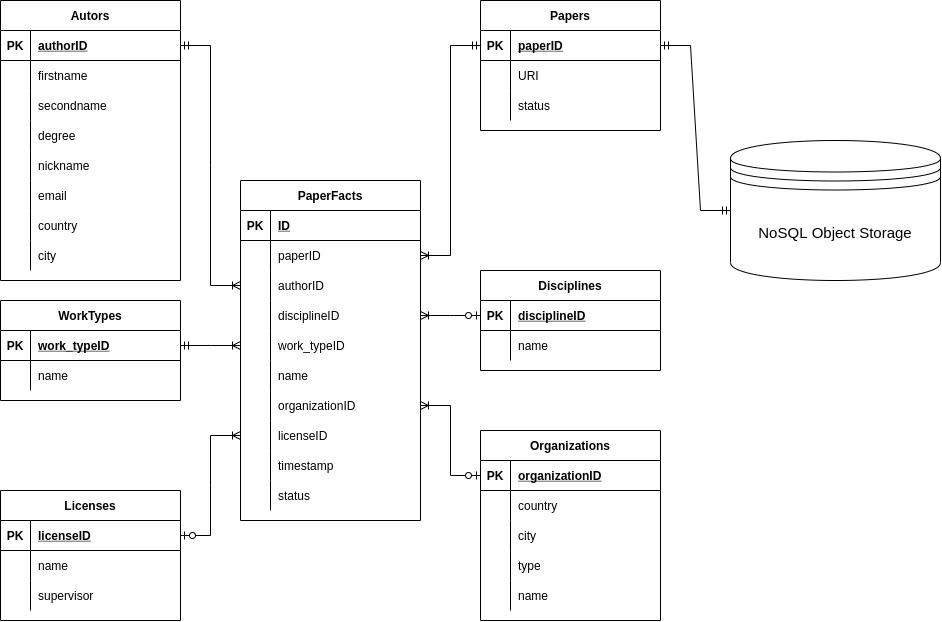
\includegraphics[width=0.8\linewidth]{images/data-model}
	\caption{ER диаграмма}
	\label{fig:data-model}
\end{figure}


Разработанный пример ER-диаграммы является примером
концептуальной диаграммы, не учитывающей особенности конкретной
СУБД. 

На основе данной концептуальной диаграммы можно построить
физическую диаграмму, которая будут учитывать такие особенности СУБД,
как допустимые типы, наименования полей и таблиц, ограничения
целостности и т.п.
Для преобразования концептуальной модели в физическую необходимо
знать, что:
\begin{enumerate}
	\item Каждая сущность в ER-диаграмме представляет собой таблицу
	базы данных;
	\item Каждый атрибут становится колонкой (полем) соответствующей
	таблицы;
	\item  В некоторых таблицах необходимо вставить новые атрибуты
	(поля), которых не было в концептуальной модели — это ключевые атрибуты 
	родительских таблиц, перемещённых в дочерние таблицы для того, чтобы
	обеспечить связь между таблицами посредством внешних ключей.
\end{enumerate}

%\section*{Вывод}
%
%В ходе данной практической работы была спроектирована и описана модель данных Подсистемы Хранения информационной системы <<Сборник лабораторных работ>>. Определена схема необходимых сущностей (таблиц) и взаимосвязь таблиц между собой. По ходу разработки Системы данная схема будет дополняться и уточняться.

\newpage
\section{Создание диаграммы состояний}
%\section{СОЗДАНИЕ ДИАГРАММЫ СОСТОЯНИЙ}

Диаграммы состояний применяются, как правило, для моделирования
поведения классов, прецедентов или системы в целом.

Составим диаграмму состояний для объекта, реализующего поиск по файлам. 

\begin{enumerate}
	\item Первым этапом выступает инициализация поискового запроса. При передаче управления этому процессу передаются параметры поиска, а на выходе данные поиска сохраняются. 
	\item Второй процесс --- выдача результатов поиска, в ходе которого пользователю предоставляется список файлов, удовлетворяющих параметрам поиска. При необходимости параметры поиска могут быть уточнены. 
	\item Последним процессом выступает обращение к объектному хранилищу данных, для того, чтобы предоставить пользователю сведения, необходимые для скачивания файла. 
\end{enumerate}

В случае, если был найден хотя бы один файл, процесс завершается успешно. Если ни один файл из объектного хранилища не удовлетворял критериям поиска, процесс завершится не успешно. Пользователю будет предложено изменить критерии поиска. 

Диаграмма состояний приведена на рисунке \ref{fig:statechart}.

% TODO: \usepackage{graphicx} required
\begin{figure}[h!]
	\centering
	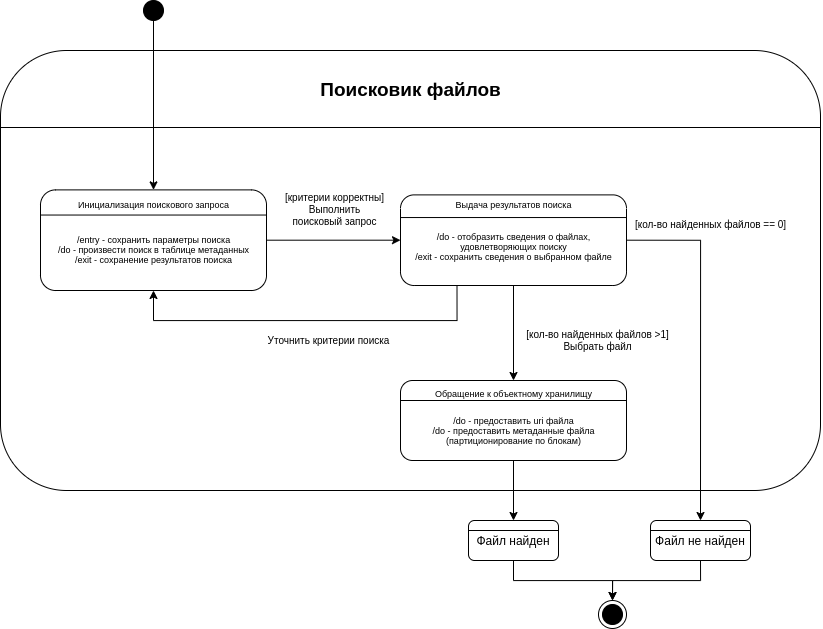
\includegraphics[width=0.6\linewidth]{images/statechart}
	\caption{Диаграмма состояний}
	\label{fig:statechart}
\end{figure}


%\section*{Вывод}
%
%В ходе данной практической работы была спроектирована и описана модель данных Подсистемы Хранения информационной системы <<Сборник лабораторных работ>>. Определена схема необходимых сущностей (таблиц) и взаимосвязь таблиц между собой. По ходу разработки Системы данная схема будет дополняться и уточняться.
%
\clearpage
\section{Расчет параметров проектируемой информационной	системы}

\subsection{ОПИСАНИЕ ЭСЕ}

Элементарная семантическая единица (ЭСЕ) --- неделимая единица
информации, использующаяся в ИС. ЭСЕ представляет собой завершенную
контекстную конструкцию, вызываемую в результате поиска по различным
атрибутам или в результате тех или иных команд в виде отклика или отчета. В случае исследования настоящей системы за элементарную семантическую единицу была выбрана одна из характеристик поиска, а именно, количество файлов, удовлетворяющим пользовательским критериям поиска. В нашем примере эта величина меняется случайным
образом в пределах от 0 до 49999 [файлов].


\subsection{НАПОЛНЕНИЕ СИСТЕМЫ}

Проектируемая информационная система <<Электронный сборник лабораторных работ>> может быть наполнена
практически любым количеством элементов базы данных. Их количество
ограничиваются только параметрами сервера.

В рамках данной практической работы система была наполнена 50000 ЭСЕ. Было проведено сто экспериментов, в ходе которых стало известно количество файлов, удовлетворяющих пользовательским параметрам, заданным в модуле поиска Подсистемы хранения ИС <<Электронный сборник лабораторных работ>>. Список результатов измерений приведен в приложении 1.


\subsection{МАТЕМАТИЧЕСКИЕ РАСЧЕТЫ}
Для дальнейшего исследования проектируемой ИС необходимо
рассчитать вероятности, с которыми ЭСЕ принимает то или иное значение.
Для оценки этих вероятностей было принято решение разбить весь диапазон
значений на 10 дискретных величин с шагом в 5000. 

Расчеты вероятности ведутся с
помощью следующей формулы  \ref{math:prob}.
\begin{align}
P(\xi)=\frac{n}N \label{math:prob}
\end{align}
В данной формуле $n$ --- благоприятное число исходов (в данном
случае число найденных файлов, попавших в данный диапазон), а $N$ --- общее число исходов. 

В таблице \ref{tab:probs} приведены возможные значения, принимаемые ЭСЕ и их вероятности.

\begin{table}[h!]
	\centering
	\caption{Ряд распределения}
	\begin{tabular}{|c|c|c|}
		\hline
		№ &	$x_i$ & $P(x)$ \\ \hline\hline
		1 &	2499.50 & 150.15 \\ \hline
		2 &		7499.50 & 100.10 \\ \hline
		3 &		12499.50 & 80.08 \\ \hline
		4 &		17499.50 & 90.09 \\ \hline
		5 &		22499.50 & 110.11 \\ \hline
		6 &		27499.50 & 130.13 \\ \hline
		7 &		32499.50 & 100.10 \\ \hline
		8 &		37499.50 & 90.09 \\ \hline
		9 &		42499.50 & 60.06 \\ \hline
		10 &		47499.50 & 90.09 \\ \hline
	\end{tabular}
	\label{tab:probs}
\end{table}

\subsubsection{Расчет математического ожидания информационного блока системы}
Математическим ожиданием случайной величины называется сумма
произведений всех возможных значений случайной величины на вероятности
этих значений. 

Рассчитаем математическое ожидание для нашей системы, взяв
за случайную величину число файлов. Расчёт математического
ожидания информационного блока на примере 10 записей:

\begin{align}
M_{x_{i}} = \sum_{i=0}^{n}\left[p_i \cdot x_i\right] \label{math:expectation}
\end{align}

\newpage
Используя данные, полученные в таблице \ref{tab:probs}, получаем:

$M(10) = 23199.50$ файлов, следовательно, наиболее вероятное
количество файлов в ответе на запрос находится в районе $23199.50$ [файлов].

\subsubsection{Расчет дисперсии информационного блока системы}

Рассчитаем дисперсию информационного блока системы по формуле \ref{math:dispers}.

\begin{align}
D_{x_i}=\sum_{i=0}^{n}\left[p_i \cdot \left(x_i\right)^2 \right] - \left[\sum_{i=0}^{n} \left(p_i \cdot x_i\right) \right]^2
\label{math:dispers}
\end{align}

Используя данные, полученные в таблице \ref{tab:probs}, получаем:

$D(10) = 206010000\mbox{ }файлов^2$

\subsubsection{Расчет среднеквадратического отклонения}

Рассчитаем среднеквадратическое отклонение по формуле \ref{math:square}.
\begin{align}
\sigma x_i= \sqrt{Dx_i} = \sqrt{206010000} = 14353.05\mbox{ файлов}	
\label{math:square}
\end{align}

\subsubsection{Расчет энтропии системы}

Информационная энтропия --- мера неопределённости некоторой системы (в статистической физике или теории информации), в частности, непредсказуемость появления какого-либо символа первичного алфавита. В последнем случае при отсутствии информационных потерь энтропия численно равна количеству информации на символ передаваемого сообщения

Вычислим энтропию системы по формуле 
\begin{align}
H(x) = - \sum_{i=1}^{n}\left[p_i \cdot \log_ap_i\right]
\end{align}

За основание логарифма a возьмем двоичную систему счисления (формула Шеннона). Энтропия фрагмента информационного наполнения в размере 10 ЭСЕ:
Используя данные, полученные в таблице \ref{tab:probs}, получаем:
$H(10) = 3.28 $ бит.

%\newpage
\subsection{РЕЗУЛЬТАТЫ РАСЧЕТОВ}

В данной главе был осуществлен расчет основных характеристик
проектируемой ИС, и получены следующие результаты:

\begin{table}[h!]
	\centering
	\caption{Параметры проектируемой ИС}
	\begin{tabular}{|p{0.6\linewidth}|p{0.4\linewidth}|}
		\hline
		Математическое ожидание информационного блока & $M(10) = 23199.50$ файлов\\\hline
		Допустимый разброс значений смысловых
		информационных блоков (дисперсия) & $D(10) = 206010000\mbox{ }файлов^2$ \\\hline
		Среднеквадратичное отклонение & $\sigma x_i=14353.05\mbox{ файлов}$	\\\hline
		Энтропия информационного наполнения & $H(10) = 3.28 $ бит \\\hline
	\end{tabular}
\end{table}
%\newpage
Приведем таблицу с исходными сгенерированными данными (см. таблицу \ref{tab:source}).
\begin{table}[h!]
	\small
	\caption{Исходные значения}
	\centering
	\begin{tabular}{|r|r|r|r|r|r|r|r|}
		\hline
		\multicolumn{1}{|l|}{№} & \multicolumn{1}{l|}{Значение} & \multicolumn{1}{l|}{№} & \multicolumn{1}{l|}{Значение} & \multicolumn{1}{l|}{№} & \multicolumn{1}{l|}{Значение} & \multicolumn{1}{l|}{№} & \multicolumn{1}{l|}{Значение} \\ \hline
		1 & 19956 & 26 & 1983 & 51 & 3986 & 76 & 47044 \\ \hline
		2 & 30937 & 27 & 26452 & 52 & 20469 & 77 & 26520 \\ \hline
		3 & 49379 & 28 & 899 & 53 & 14592 & 78 & 35967 \\ \hline
		4 & 32802 & 29 & 41888 & 54 & 1352 & 79 & 21749 \\ \hline
		5 & 3998 & 30 & 8182 & 55 & 32704 & 80 & 18295 \\ \hline
		6 & 31012 & 31 & 2176 & 56 & 40990 & 81 & 21813 \\ \hline
		7 & 38782 & 32 & 28627 & 57 & 29975 & 82 & 13467 \\ \hline
		8 & 15895 & 33 & 25433 & 58 & 10325 & 83 & 23783 \\ \hline
		9 & 27847 & 34 & 9457 & 59 & 3700 & 84 & 32821 \\ \hline
		10 & 35964 & 35 & 2373 & 60 & 24083 & 85 & 17607 \\ \hline
		11 & 3827 & 36 & 10010 & 61 & 33412 & 86 & 36274 \\ \hline
		12 & 24247 & 37 & 48230 & 62 & 43067 & 87 & 10648 \\ \hline
		13 & 39557 & 38 & 26061 & 63 & 49735 & 88 & 19679 \\ \hline
		14 & 2321 & 39 & 5810 & 64 & 40199 & 89 & 49114 \\ \hline
		15 & 29616 & 40 & 25460 & 65 & 20796 & 90 & 43305 \\ \hline
		16 & 24485 & 41 & 30058 & 66 & 27099 & 91 & 21310 \\ \hline
		17 & 46153 & 42 & 859 & 67 & 36430 & 92 & 31711 \\ \hline
		18 & 35865 & 43 & 46295 & 68 & 18874 & 93 & 18424 \\ \hline
		19 & 44427 & 44 & 1274 & 69 & 6761 & 94 & 6493 \\ \hline
		20 & 26134 & 45 & 37563 & 70 & 8725 & 95 & 5029 \\ \hline
		21 & 2133 & 46 & 47881 & 71 & 25199 & 96 & 9433 \\ \hline
		22 & 3270 & 47 & 15273 & 72 & 21981 & 97 & 38202 \\ \hline
		23 & 27499 & 48 & 1346 & 73 & 48131 & 98 & 33052 \\ \hline
		24 & 33954 & 49 & 11422 & 74 & 13900 & 99 & 24332 \\ \hline
		25 & 17943 & 50 & 11215 & 75 & 6764 & 100 & 5224 \\ \hline
	\end{tabular}
	\label{tab:source}
\end{table}


\section{Вывод}

В ходе выполнения данных практических работ был разработан комплект документов, описывающих выбранную к разработке информационную систему <<Электронный сборник лабораторных работ>>. Были сформированы требования к системе, определены цели, которые необходимо достичь и задачи, которые призвана решить информационная система, описаны сценарии использования; с учетом требований и ограничений было выбрано программное обеспечение, которое будет использовано при разработке проектируемой системы.

Были разработаны структурные диаграммы в различных~нотациях~---~UML, IDEF0, DFD, ER. Также был произведен расчет параметров проектируемой информационной системы. 

\end{document}

